\documentclass[letterpaper, 12pt]{article}
\usepackage{geometry}
\geometry{
    letterpaper,
    left=20mm,
    top=20mm,
    bottom=20mm
}
\usepackage{tocloft}
\usepackage{graphicx}
\usepackage{authblk}
\usepackage{amssymb}
\usepackage{lipsum}
\usepackage{float}
\usepackage{times}
\usepackage{amsmath}
\usepackage[format=plain,
            labelfont={bf,it},
            textfont=it]{caption}
\captionsetup{justification=raggedright,singlelinecheck=false}
\usepackage{ragged2e}
\usepackage{longtable}
\usepackage{comment}
\usepackage{setspace}
\usepackage{fancyhdr}
\usepackage{titlesec}
\usepackage[hyperindex,breaklinks]{hyperref}
\hypersetup{
    colorlinks=true,
    linkcolor=blue,
    filecolor=magenta,      
    urlcolor=blue
}
\usepackage[T1]{fontenc}
\usepackage{helvet}
\renewcommand{\familydefault}{\sfdefault}
\pagenumbering{gobble}
\usepackage[skip=10pt plus1pt, indent=40pt]{parskip}
\usepackage{orcidlink}
\usepackage{standalone}

\titlespacing*{\section}
{0pt}{1.5ex plus 1ex minus .2ex}{1.3ex plus .2ex}

\renewcommand\Authfont{\fontsize{12}{14.4}\selectfont}
\renewcommand\Affilfont{\fontsize{9}{10.8}\itshape}

\newcommand{\cosigpart}[1]{
  \addcontentsline{toc}{part}{#1}
}
\newcommand{\cosigsection}[1]{
  \section*{#1}
  \phantomsection % avoid warnings from hyperref about the anchor of a bookmark and its parent's
  \addcontentsline{toc}{section}{#1}
}
\begin{document}
\flushleft
\includegraphics[width=0.5\textwidth]{img/home/241017_final_logo_mockup.png}

\cosigsection{Extracting vector graphics from a PDF}
\textit{Last updated: 19 May 2025}

It is often difficult to tell if two line graphs have shared features from a published figure alone. While the webpage of a scientific article invariable displays these images in raster format (i.e. pixel-based), the PDF version of the article may actually display these images in vector format, meaning that the features of the figure can be more easily magnified and compared.

An easy way to check if a figure in the PDF of a scientific article is in raster format or vector format is to try highlighting the text in the figure with your cursor (e.g. the text that labels the axes of the graph). If the text within the figure can be highlighted, the image is probably in vector format. Consider \href{https://doi.org/10.1007/s12182-020-00439-9}{this article}, for which the figures in the PDF are in vector format, and \href{https://doi.org/10.1016/j.est.2023.109227}{this article}, for which the images in the PDF are in raster format.

\begin{figure}[h!tbp]
    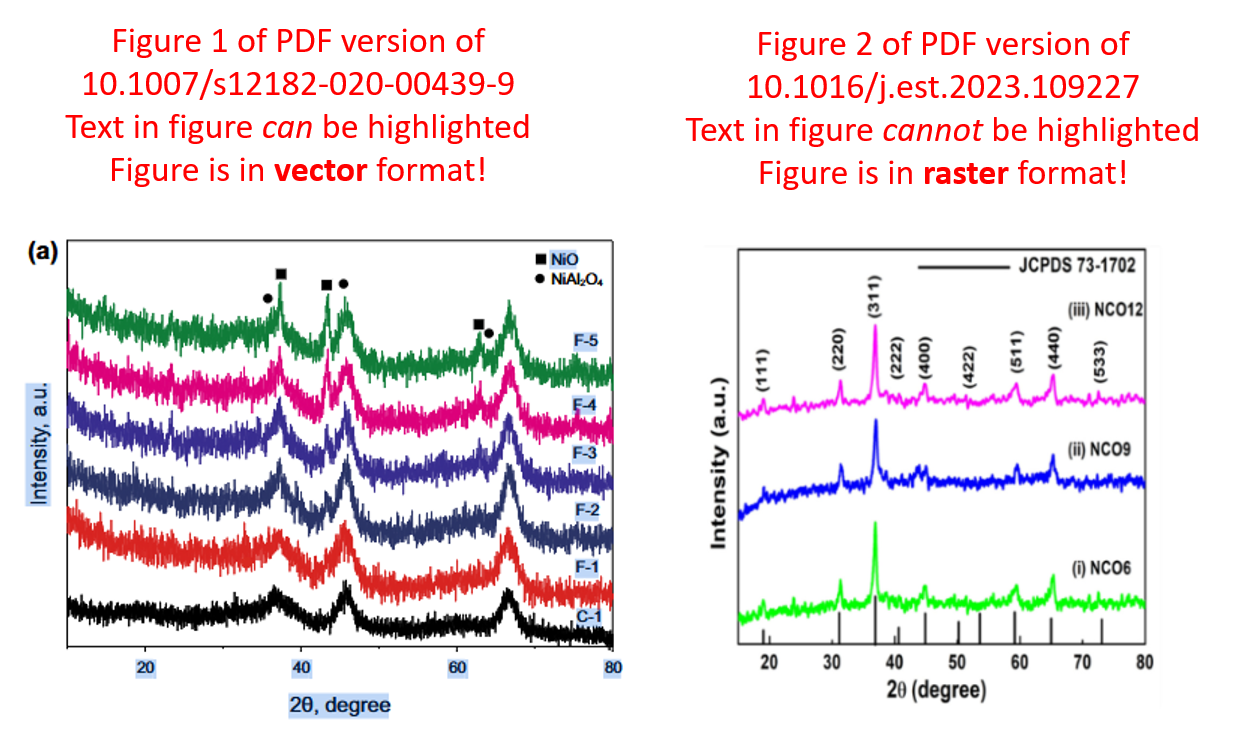
\includegraphics[width=\textwidth]{img/vector/vector_vs_raster.png}
    \caption*{ The figure on the left is embedded within its PDF in vector format, whereas the image on the right is embedded within its PDF in raster format.}
\end{figure}

Vector graphics can be isolated in any vector graphics editor like \href{https://www.adobe.com/products/illustrator.html}{Adobe Illustrator} or its free, open-source alternative \href{https://inkscape.org/}{Inkscape}. We'll use Inkscape for this demonstration but the procedure will be more or less the same in other vector graphics editors.

First, open Inkscape, navigate to \textbf{File > Open}, and select your PDF of interest. For this demonstration, we'll use Figure 1B in the PDF of \href{https://doi.org/10.1007/s12182-020-00439-9}{this article}. After the PDF opens, scroll over to your figure of interest and select your component of interest.

\begin{figure}[h!tbp]
    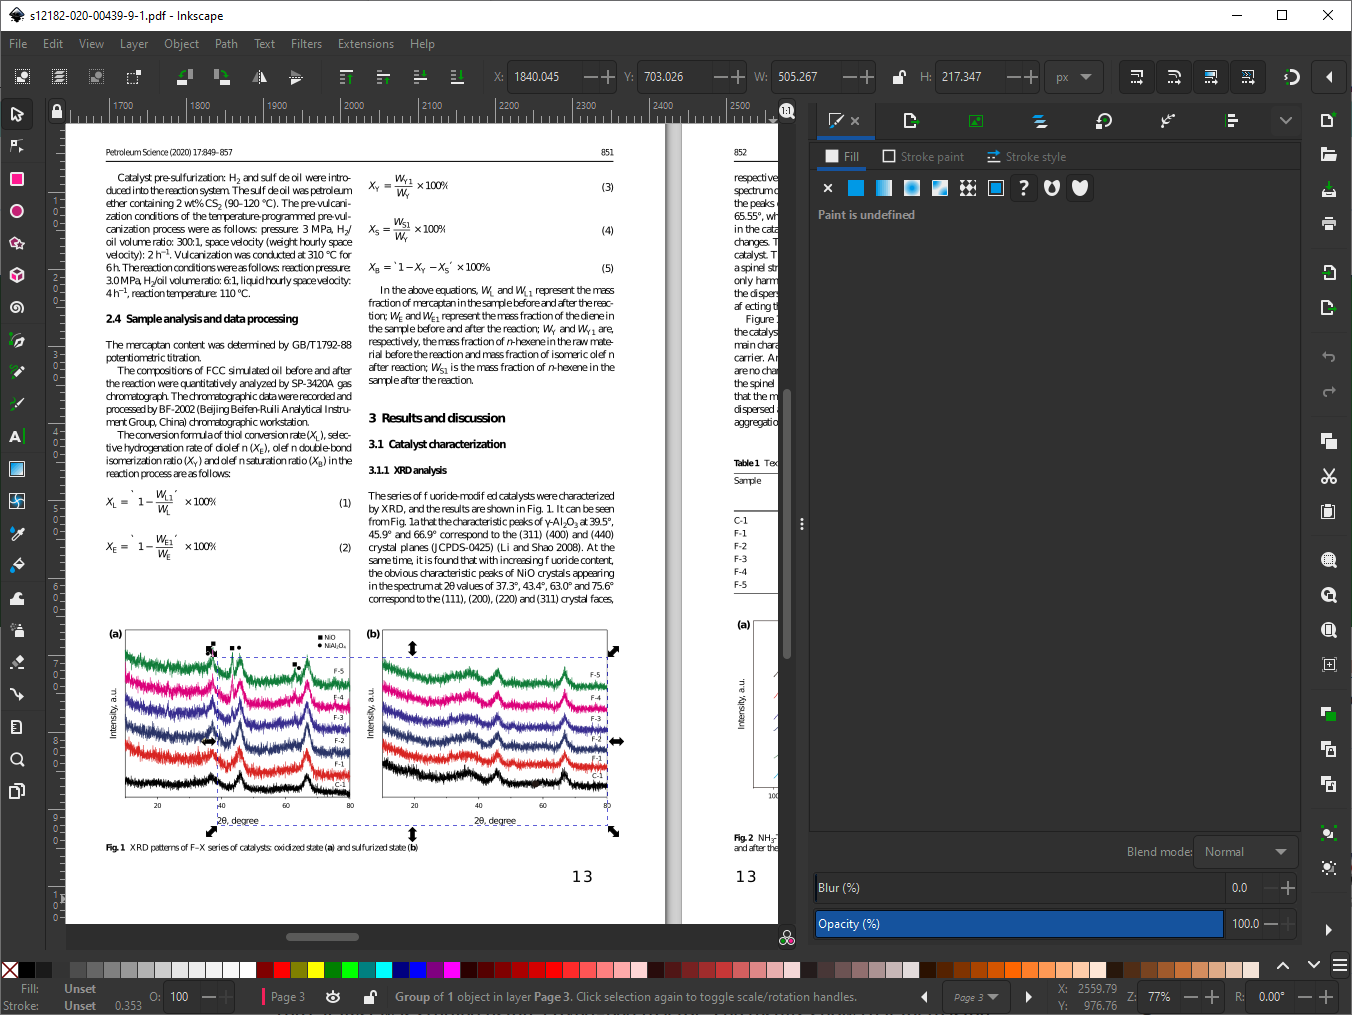
\includegraphics[width=\textwidth]{img/vector/in_inkscape.png}
    \caption*{Our PDF opened in Inkscape with the traces in Figure 1B selected.}
\end{figure}

\pagebreak
Next, repeatedly use \textbf{Right click > Ungroup (Shift + Ctrl + G)} on the selected objects until individual objects (in this case, individual line traces) can be selected.

\begin{figure}[h!tbp]
    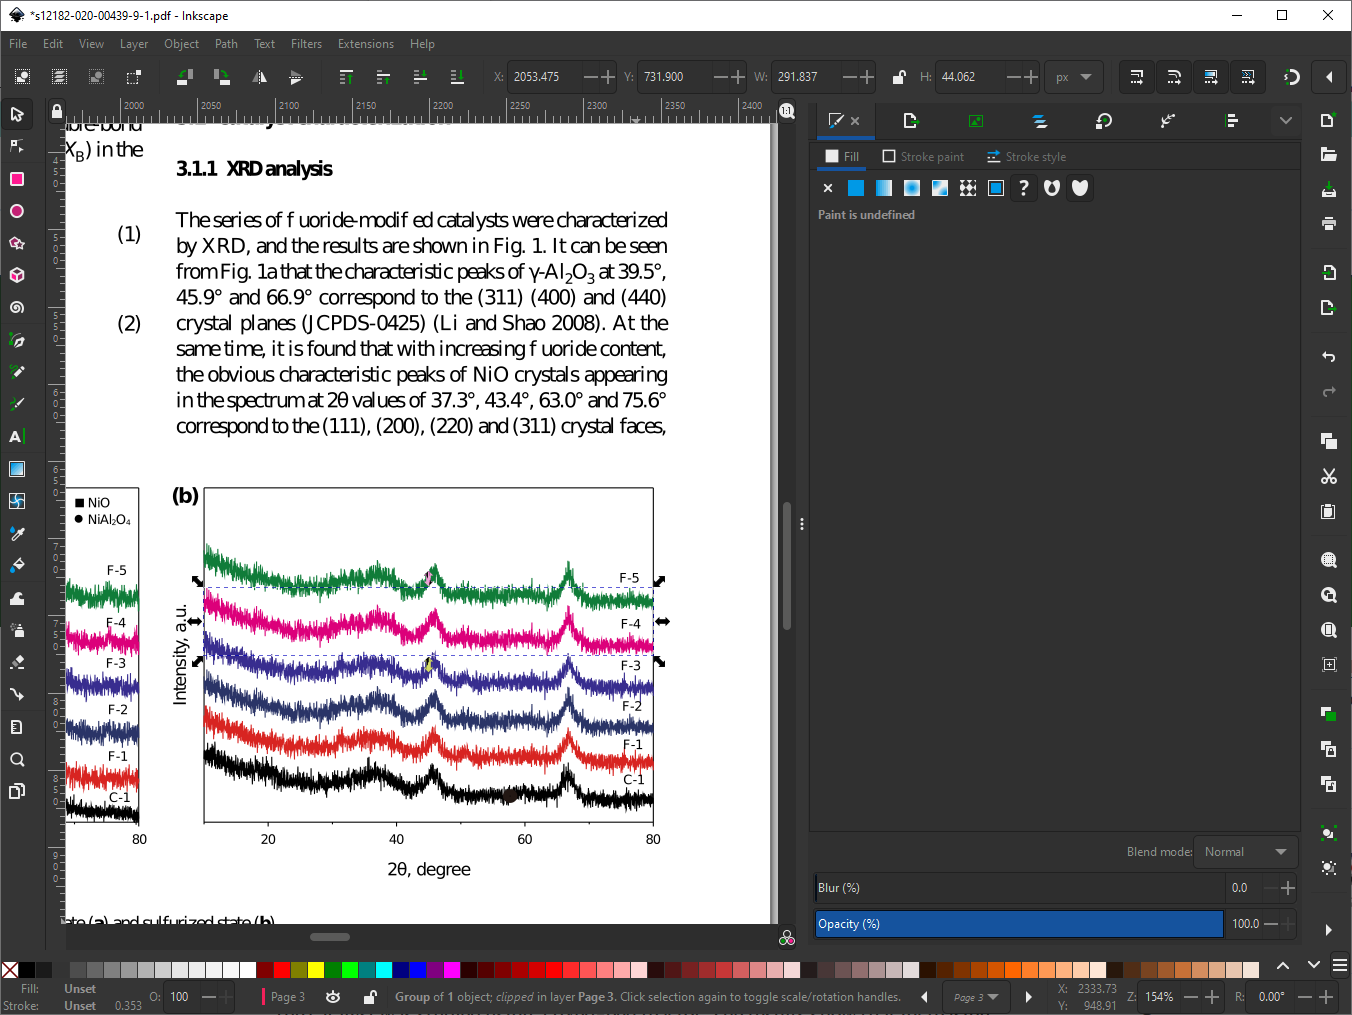
\includegraphics[width=\textwidth]{img/vector/in_inkscape_individual_traces.png}
    \caption*{After repeatedly ungrouping objects, we can now select individual line traces.}
\end{figure}

\pagebreak
When viewing line traces, it is helpful, but not necessary, to thin out the traces to enable comparison. To do so, navigate to \textbf{Objects > Fill and Stroke (Shift + Ctrl + F)}, under which the \textbf{Stroke Style} menu allows you to set line thickness. Afterwards, moving the traces to be closer to one another reveals that the F-2 (navy), F-4 (pink) and F-5 (green) traces are identical and the F-3 (blue) and F-1 (red) traces are identical.

\begin{figure}[h!tbp]
    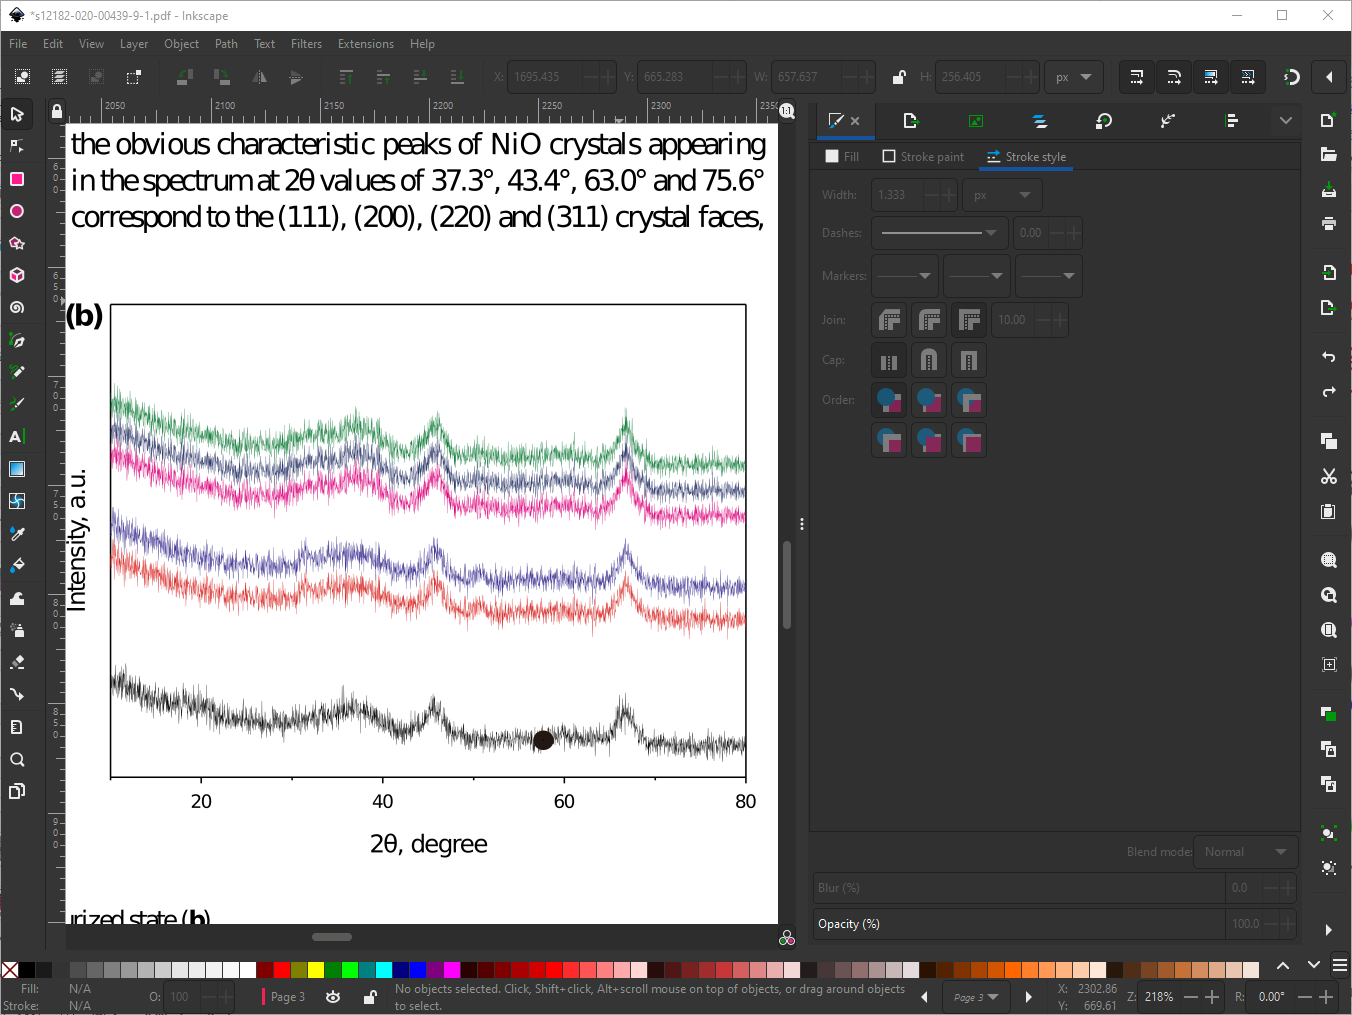
\includegraphics[width=\textwidth]{img/vector/in_inkscape_individual_traces_thinned.png}
    \caption*{Moving around and thinning out traces in Inkscape allows for easier comparison.}
\end{figure}

\pagebreak
We can also overlap the traces to make it crystal clear that these are the same data.

\begin{figure}[h!tbp]
    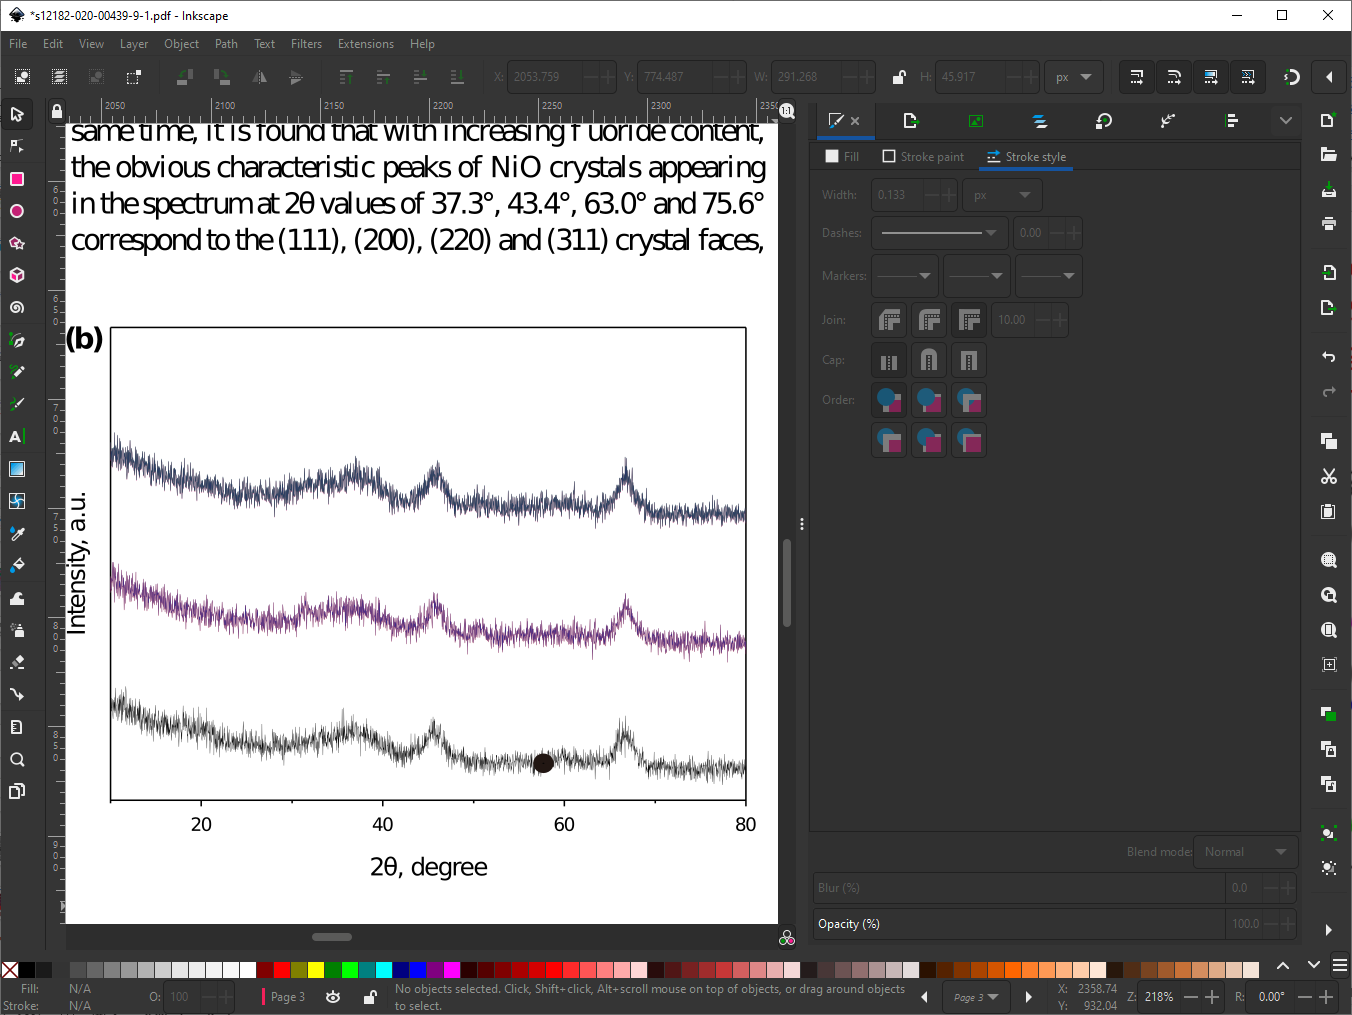
\includegraphics[width=\textwidth]{img/vector/in_inkscape_individual_traces_thinned_overlapping.png}
    \caption*{Now that traces are individual objects, we can easily overlap them to show that certain traces are identical.}
\end{figure}

\pagebreak
Objects can also be copy-pasted into a new document.

\begin{figure}[h!tbp]
    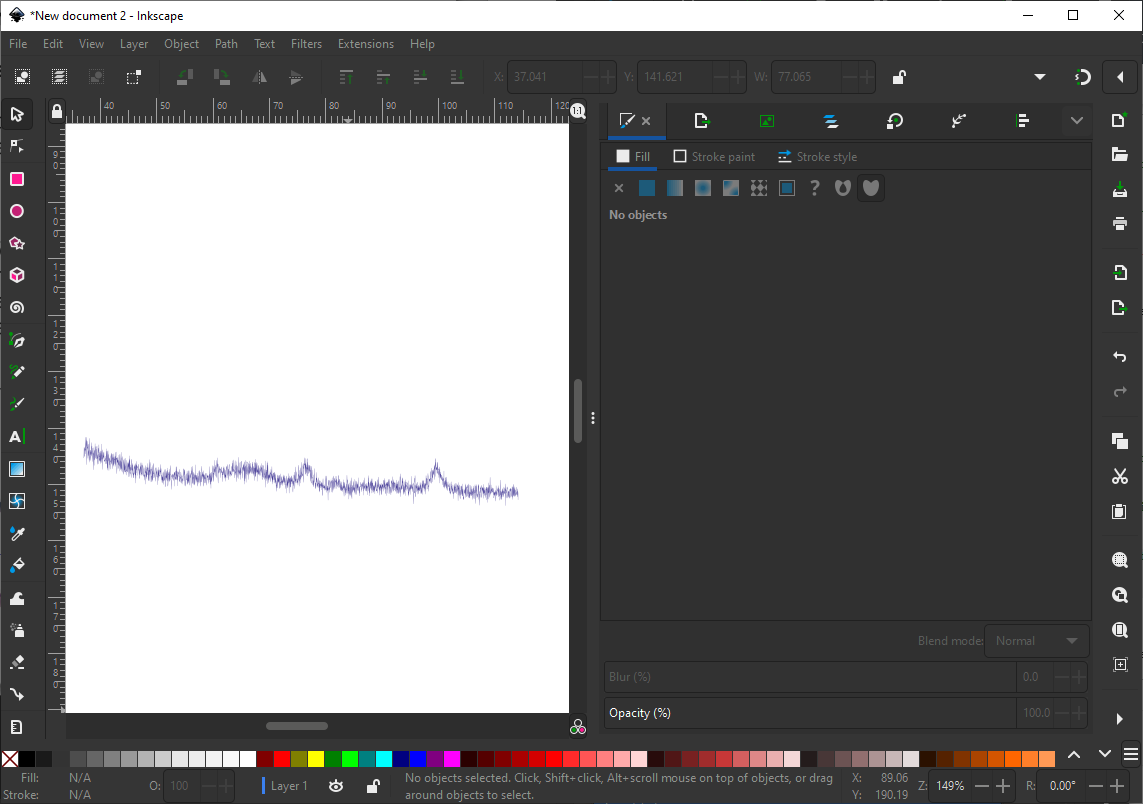
\includegraphics[width=\textwidth]{img/vector/inkscape_new_document.png}
    \caption*{ An individual trace copied into a new Inkscape document.}
\end{figure}

To practice, try extracting graphical elements from the vector figures in \href{https://osf.io/gpxvf}{COSIG's entry on Tauc plots} or \href{https://osf.io/685xa}{COSIG's entry on data duplication in X-ray diffraction patterns}.

\end{document}
